\section{最大值原理}
\label{sec:ellip-maximum}

前面的能量估计控制的是平方积分的大小，没有告诉我们解在哪里最大。温度分布有一个直观的事实：没有内部热源时，最高温只能出现在边界上。若内部出现了一个比周围都热的点，热量就会从它流向四周，无法平衡。把这个直觉变成定理，需要用到方程的符号结构。

\paragraph{调和函数是平均值}
上面的直觉有一个精确的版本：调和函数在每一点的值，等于以该点为心的任意球面上的平均值，这称为\term{平均值性质}（mean value property）。

\begin{theorem}[平均值性质]
\label{thm:ellip-mean-value}
设$u\in C^2(\Omega)$在$\Omega$内调和，$\overline{B_r(\bm{x})}\subset\Omega$。则
\begin{equation}
 u(\bm{x})=\frac1{\lvert\partial B_r\rvert}\int_{\partial B_r(\bm{x})}u\,\mathrm{d}S,
 \label{eq:ellip-mean-value}
\end{equation}
并且对球体上的平均，同样的等式成立。
\end{theorem}

\begin{proof}
把球面积分写成单位球面$S$上的平均，令
\[
 m(r)=\frac1{\lvert S\rvert}\int_Su(\bm{x}+r\bm{\omega})\,\mathrm{d}\sigma(\bm{\omega}) .
\]
对$r$求导，换回半径$r$的球面，并用散度定理：
\[
 m'(r)=\frac1{\lvert\partial B_r\rvert}\int_{\partial B_r}\partial_{\bm{n}}u\,\mathrm{d}S=\frac1{\lvert\partial B_r\rvert}\int_{B_r}\Delta u\,\mathrm{d}\bm{y}=0 .
\]
所以$m$是常数，又因$u$连续，$r\to0$时$m(r)\to u(\bm{x})$。这就证明了式~\eqref{eq:ellip-mean-value}。球体上的平均是不同半径的球面平均对$r$的加权积分，也等于$u(\bm{x})$。
\end{proof}

图~\ref{fig:ellip-harmonic-saddle}中，$u=x_1^2-x_2^2$在圆盘上调和。圆周上的值有高有低，平均后恰好是圆心的值。这个函数的最大值出现在边界上的两个红点，最小值在两个紫点，内部的鞍点不是极值。

\begin{BookInlineFigure}
  \centering
  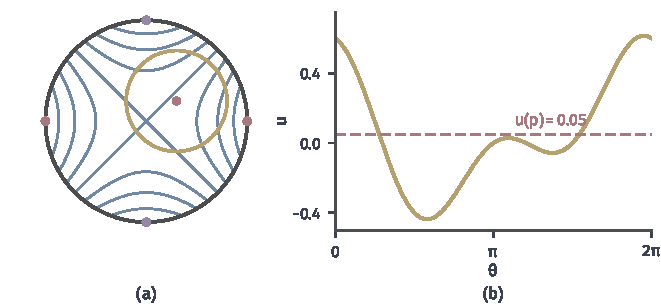
\includegraphics[width=112mm]{figures/06-differential-equations/02-partial-differential-equations/matplotlib/ellip-harmonic-saddle/figure.pdf}
  \caption{调和函数$u=x_1^2-x_2^2$。(a)单位圆盘内的等值线，红点是边界上的最大值点，紫点是最小值点。黄圆心在$\bm{p}=(0.3,0.2)$，半径$0.5$。(b)黄圆上$u$的取值（黄），红色虚线是圆心值$u(\bm{p})=0.05$，也是这些取值的平均值。}
  \label{fig:ellip-harmonic-saddle}
\end{BookInlineFigure}

\paragraph{Laplace算子的最大值原理}
把“内部的值不超过边界上的值”写成定理，就是\term{最大值原理}（maximum principle）。它只要求$-\Delta u\leq0$，即区域内部没有热源，但可以有热汇。

\begin{theorem}[弱最大值原理]
\label{thm:ellip-weak-max}
设$\Omega$是有界开集，$u\in C^2(\Omega)\cap C(\overline\Omega)$，在$\Omega$内$-\Delta u\leq0$。则
\begin{equation}
 \max_{\overline\Omega}u=\max_{\partial\Omega}u.
 \label{eq:ellip-weak-max}
\end{equation}
\end{theorem}

\begin{proof}
先处理严格的情形。若$-\Delta v<0$，$v$不可能在内部取最大值：在内部最大值点，每个方向的二阶导数都不超过零，$\Delta v\leq0$，与$\Delta v>0$矛盾。

对一般的$u$，令$v_\varepsilon=u+\varepsilon\lVert\bm{x}\rVert_2^2$，$\varepsilon>0$。则$\Delta v_\varepsilon=\Delta u+2d\varepsilon>0$，所以$v_\varepsilon$的最大值在边界上取得，于是
\[
 \max_{\overline\Omega}u\leq\max_{\overline\Omega}v_\varepsilon=\max_{\partial\Omega}v_\varepsilon\leq\max_{\partial\Omega}u+\varepsilon\max_{\partial\Omega}\lVert\bm{x}\rVert_2^2 .
\]
令$\varepsilon\to0$，得到$\max_{\overline\Omega}u\leq\max_{\partial\Omega}u$。反向不等式由$\partial\Omega\subset\overline\Omega$得到。
\end{proof}

定理说最大值在边界上取得，但不排除内部也取到。调和函数的情形可以说得更多：若$\Omega$连通，调和函数在内部取到最大值，则必为常数。设最大值$M$在内部某点取到，集合$\{u=M\}$在$\Omega$中闭。由球上的平均值性质，若$u(\bm{x})=M$，球内$u\leq M$而平均等于$M$，只能处处等于$M$，所以这个集合又是开的。连通性使它等于整个$\Omega$。这是强最大值原理在调和情形的证明。

\paragraph{比较与上界}
最大值原理最直接的用途是比较两个解。把定理用于差$u-w$，得到\term{比较原理}（comparison principle），再选择不同的比较函数，就有下面三个结论。

\begin{theorem}[比较原理与上界]
\label{thm:ellip-comparison}
设$\Omega$是有界开集，$u,w\in C^2(\Omega)\cap C(\overline\Omega)$。
\begin{enumerate}
 \item 若在$\Omega$内$-\Delta u\leq-\Delta w$，在$\partial\Omega$上$u\leq w$，则在$\Omega$内$u\leq w$。
 \item Poisson方程的Dirichlet问题最多有一个$C^2(\Omega)\cap C(\overline\Omega)$解。
 \item 设$\Omega\subset B_\rho(\bm{x}_0)$，$-\Delta u=f$，$u=g$于$\partial\Omega$，且$f$有界。则
 \begin{equation}
 \max_{\overline\Omega}\lvert u\rvert\leq\max_{\partial\Omega}\lvert g\rvert+\frac{\rho^2}{2d}\sup_\Omega\lvert f\rvert .
 \label{eq:ellip-max-bound}
 \end{equation}
\end{enumerate}
\end{theorem}

\begin{proof}
第1条，$z=u-w$满足$-\Delta z\leq0$，由定理~\ref{thm:ellip-weak-max}，$\max z=\max_{\partial\Omega}z\leq0$。第2条，两个解的差$z$满足$\Delta z=0$且边界值为零，把定理用于$z$与$-z$，得到$z=0$。

第3条，记$F=\sup\lvert f\rvert$，$G_0=\max_{\partial\Omega}\lvert g\rvert$。取比较函数
\[
 w(\bm{x})=G_0+\frac F{2d}\bigl(\rho^2-\lVert\bm{x}-\bm{x}_0\rVert_2^2\bigr).
\]
由$\Delta\lVert\bm{x}\rVert_2^2=2d$，$-\Delta w=F\geq\pm f$，并且$\overline\Omega$上$w\geq G_0\geq\pm g$。第1条分别用于$u$和$-u$，得到$\lvert u\rvert\leq w\leq G_0+F\rho^2/(2d)$。
\end{proof}

检验一下估计的精度。$\Omega=(0,1)$，$d=1$，$\rho=1/2$，$\bm{x}_0=1/2$，$f=1$，$g=0$，式~\eqref{eq:ellip-max-bound}给出$\lvert u\rvert\leq1/8$，恰好等于真解的最大值。这里比较函数$w=\frac12(\frac14-(x-\frac12)^2)=x(1-x)/2$就是真解本身。

比较原理还告诉我们，$f\geq0$且$g\geq0$时$u\geq0$，即加热不会使温度降低。这对点源同样成立，所以Green函数非负：$G(\bm{x},\bm{y})\geq0$，在式~\eqref{eq:ellip-green-1d}中也能直接看出来。

\paragraph{带低阶项的算子}
考虑更一般的算子，写成非散度形式
\begin{equation}
 Lu=-\operatorname{tr}\bigl(\bm{A}\nabla^2u\bigr)+\bm{b}\cdot\nabla u+cu,
 \label{eq:ellip-general-operator}
\end{equation}
其中$\bm{A}(\bm{x})$对称，满足式~\eqref{eq:ellip-uniform}，$\bm{b}$和$c$在$\Omega$上有界，$\nabla^2u$是Hessian矩阵。式~\eqref{eq:ellip-divergence-form}在$\bm{A}\in C^1$时也能写成这个形式。

最大值原理成立的关键是$c$的符号。在正的最大值点，$\nabla u=0$，$\nabla^2u$半负定，所以$-\operatorname{tr}(\bm{A}\nabla^2u)\geq0$。若$c\geq0$，还有$cu\geq0$，两项都迫使$Lu\geq0$，这与$Lu<0$矛盾。

\begin{theorem}[带零阶项的最大值原理]
\label{thm:ellip-general-max}
设$\Omega$是有界开集，$L$如式~\eqref{eq:ellip-general-operator}，$c\geq0$。若$u\in C^2(\Omega)\cap C(\overline\Omega)$满足$Lu\leq0$，则
\begin{equation}
 \max_{\overline\Omega}u\leq\max_{\partial\Omega}u^+,
 \label{eq:ellip-general-max}
\end{equation}
其中$u^+=\max(u,0)$。若$c\equiv0$，则$\max_{\overline\Omega}u=\max_{\partial\Omega}u$。
\end{theorem}

\begin{proof}
先设$c\equiv0$，记此时的算子为$L_0$。若$L_0v<0$，由上面的论证，$v$在内部没有最大值点。一般情形下取$\gamma$足够大，令$\psi=\mathrm{e}^{\gamma x_1}$，有
\[
 L_0\psi=\bigl(-A_{1,1}\gamma^2+b_1\gamma\bigr)\psi\leq\gamma\bigl(-\kappa_{\min}\gamma+\lVert\bm{b}\rVert_\infty\bigr)\psi<0 .
\]
于是$v_\varepsilon=u+\varepsilon\psi$满足$L_0v_\varepsilon<0$，最大值在边界上取得。令$\varepsilon\to0$，与定理~\ref{thm:ellip-weak-max}的做法相同，得到结论。

再看$c\geq0$。若$u\leq0$，式~\eqref{eq:ellip-general-max}已成立。否则令$\Omega^+=\{\bm{x}\in\Omega:u(\bm{x})>0\}$。在这个开集上$L_0u=Lu-cu\leq0$，把已证结论用于$\Omega^+$。$\Omega^+$的边界点要么在$\partial\Omega$上，要么满足$u=0$，所以$u$的最大值不超过$\max_{\partial\Omega}u^+$。
\end{proof}

图~\ref{fig:ellip-sign-failure}显示$c$的两种符号。(a)中$c\geq0$，$-u''+cu=1$，$u(0)=u(1)=0$。常数函数$w=1/c$满足$Lw=1$，边界上$w>u$，由比较原理（对差$u-w$用定理~\ref{thm:ellip-general-max}）得到$u\leq1/c$，图中的点线就是这个上界。$c$越大，方程越像$cu=1$，解越贴近$1/c$。

(b)中$c=-\pi^2$，方程$-u''-\pi^2u=0$有非零解$A\sin(\pi x)$，它们的边界值都是零，内部却有非零的值，最大值原理和唯一性同时失效。这里$-\pi^2$恰好是$-\lambda_1$，用谱展开的语言说，算子有了零特征值。

\begin{BookInlineFigure}
  \centering
  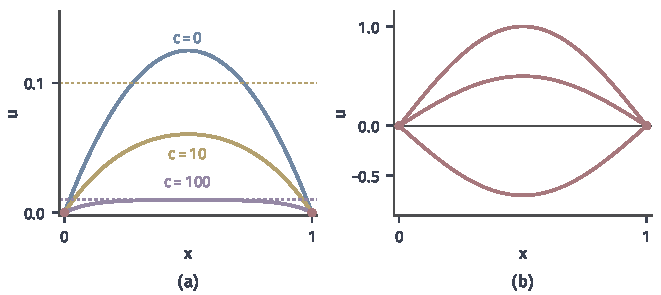
\includegraphics[width=112mm]{figures/06-differential-equations/02-partial-differential-equations/matplotlib/ellip-sign-failure/figure.pdf}
  \caption{零阶项的符号。(a)$-u''+cu=1$，零边界，$c=0,10,100$，点线是上界$u\leq1/c$（$c=0$时无此上界）。(b)$c=-\pi^2$时$u=A\sin(\pi x)$（红线，$A=1,\tfrac12,-\tfrac7{10}$）都满足齐次方程和零边界，最大值原理失效。}
  \label{fig:ellip-sign-failure}
\end{BookInlineFigure}

\paragraph{弱解的最大值原理}
定理~\ref{thm:ellip-general-max}要求$u\in C^2$。散度型方程的弱解有一个不需要二阶导数的版本，它把能量方法和最大值原理连在了一起。

设$u\in H^1(\Omega)$是式~\eqref{eq:ellip-divergence-form}的弱解，$f\leq0$，$\operatorname{Tr}u\leq M$。把$v=(u-M)^+$作为测试函数，这里用到$H^1$函数被截断后仍在$H^1$中，且$\nabla v=\nabla u\,\mathbf{1}_{\{u>M\}}$，$v$的迹为零，所以$v\in H^1_0(\Omega)$。

由弱形式和$f\leq0$，$v\geq0$，
\[
 \kappa_{\min}\lVert\nabla v\rVert_2^2\leq\int_\Omega\bm{A}\nabla v\cdot\nabla v\,\mathrm{d}\bm{x}=a(u,v)=\int_\Omega fv\,\mathrm{d}\bm{x}\leq0 .
\]
所以$\nabla v=0$，由Poincaré不等式$v=0$，即$u\leq M$几乎处处成立。这个证明不要求$\bm{A}$连续，也适用于前面那根两段材料的棒。

\paragraph{两种估计的对比}
能量估计与最大值估计回答不同的问题，见表~\ref{tab:ellip-energy-vs-max}。两者不能互相替代：弱解的能量估计不给出逐点的界，而最大值原理不给出梯度的积分界。

\begin{BookInlineTable}
  \centering
  \caption{能量估计与最大值估计的对比。}
  \label{tab:ellip-energy-vs-max}
  \begin{tabular}{lll}
    \toprule
    & 能量估计 & 最大值估计\\
    \midrule
    控制的量 & $\lVert\nabla u\rVert_2$（平方平均） & $\max\lvert u\rvert$（逐点）\\
    数据的度量 & $\lVert f\rVert_2$ & $\sup\lvert f\rvert$\\
    结构要求 & 强制性 & 符号（$c\geq0$）\\
    适用范围 & 方程组同样可用 & 只对标量方程\\
    \bottomrule
  \end{tabular}
\end{BookInlineTable}
